\documentclass[11pt]{article}
\usepackage[margin=1in]{geometry}
\usepackage{amsmath,amssymb,amsthm,bm}
\usepackage{graphicx}
\usepackage{booktabs}
\usepackage{xcolor}
\usepackage[colorlinks=true,linkcolor=blue,citecolor=blue,urlcolor=blue]{hyperref}
\usepackage{caption}
\captionsetup{font=small,labelfont=bf}

\newtheorem{theorem}{Theorem}
\newtheorem{proposition}{Proposition}
\newtheorem{definition}{Definition}

\newcommand{\Pen}{\mathrm{Pe}}
\newcommand{\Trr}{\operatorname{Tr}}
\newcommand{\M}{\mathcal{M}}
\newcommand{\s}{\bm{s}}
\newcommand{\z}{\bm{z}}
\newcommand{\x}{\bm{x}}
\newcommand{\rr}{\bm{r}}

\title{\bf Coordinate-invariant routing coordinates for multi-physics machine
learning: what the geometry of the operating manifold does, and does not, buy}
\author{Sehaj Singh}
\date{\today}

\begin{document}
\maketitle

\begin{abstract}
\noindent
Machines trace trajectories through coupled thermal, mechanical and electrical
state spaces, and one global network must serve every regime along the way. A
natural proposal is to route computation on the local geometry of that space.
We formalise the proposal and test it. For a diffusion the canonical metric is
$g=V^{-1}$, the inverse diffusion tensor, so volatility is not a feature
sitting alongside curvature: it \emph{is} the geometry. The routing coordinates
then reduce to two scalars, the scalar curvature $R$ and a drift-to-noise
P\'eclet number $\Pen$, both invariant under smooth relabelling of the sensors.
We prove an exact identity governing how sharply an operator assembly may
switch and verify it to $2\times10^{-17}$. Across five systems --- a 1.3\,M
sample permanent-magnet motor bench, NASA C-MAPSS, and three MuJoCo Menagerie
arms carrying injected joint thermal networks --- geometric routing does
\emph{not} improve in-distribution accuracy over routing on the raw state at
matched capacity. $\Pen$ survives a coordinate change almost exactly
($\rho=0.999$) while the curvature does not ($\rho=0.60$), and where increments
are a jump process rather than a diffusion the metric is misspecified and
geometric routing is actively worse. We report where the construction earns its
cost and where it does not.
\end{abstract}

\section{Introduction}

A machine under load does not sit at an operating point; it moves along one.
A servo joint accelerating a payload dissipates ohmic heat into a winding whose
rising temperature derates the torque available to the next command, on a
thermal time constant three decades slower than the control loop that issued
it. A traction motor's rotor temperature, which no production sensor can reach,
is a functional of the whole recent history of current and speed. In both
cases the quantity to be predicted depends on where the machine is on a coupled
multi-physics trajectory, and a single monolithic network must serve every part
of that trajectory at once.

Mixture-of-experts routing is the standard answer, and it has been applied to
exactly these problems: multi-gate mixtures for turbofan remaining-useful-life,
fault-mode gating, regime-conditioned prognostics. In all of these the router
reads the raw state. A second, separate literature routes on \emph{geometry},
but in graph representation learning, where discrete Ollivier--Ricci curvature
selects among embedding spaces of different constant curvature. Nothing yet
routes physical computation on the intrinsic geometry of an estimated
continuous state manifold.

That is the proposal we formalise and test. The intuition is appealing: regions
where trajectories separate quickly, or where noise dominates drift, are
physically distinct and might deserve distinct computation. The intuition also
makes a sharper and more testable promise than accuracy. Curvature is a
coordinate invariant. If routing decisions are functions of invariants, they
are unchanged when the sensors are relabelled --- recalibrated, rescaled,
nonlinearly warped --- whereas a router reading the raw state is not. Fleets
are recalibrated constantly. This is the claim worth testing, and it is the one
we test.

Our contributions are as follows.

\begin{enumerate}
\item \textbf{The volatility is the metric.} Treating curvature and volatility
as two features to concatenate double-counts. For a non-degenerate diffusion
the canonical metric is $g=V^{-1}$, in which Varadhan's short-time heat-kernel
asymptotics give geodesic distance. The routing coordinates collapse to two
scalars, and become $\sim\!100\times$ cheaper to compute
(Section~\ref{sec:theory}).
\item \textbf{An exact switching identity.} The sensitivity of an assembly to
its routing coordinate is exactly a gate-weighted covariance between router
logit gradients and expert outputs (Theorem~\ref{thm:sens}); verified to
$2\times10^{-17}$.
\item \textbf{A negative in-distribution result, with controls.} At matched
parameter count, matched expert bank and matched expert inputs --- so that only
the router's input differs --- geometric routing does not beat raw-state
routing on any of five systems. Controls for dimensionality, for basis
dependence and for cheap non-geometric proxies are all run.
\item \textbf{A diagnosis.} $\Pen$ is estimable and invariant; $R$ is
theoretically the more attractive coordinate and empirically the less reliable
one, because it is a second derivative of an estimated diffusion field. Where
increments are jumps rather than diffusion, the whole construction is
misspecified and we show it failing.
\end{enumerate}

\section{The construction}
\label{sec:theory}

\subsection{State manifold and chart}

Let the operating state be $\s(t)\in\M\subset\mathbb{R}^d$, collecting the
measured thermal, mechanical and electrical channels. A chart
$\phi:\M\to\mathbb{R}^k$ with $k\ll d$ carries the ambient sensor vector to
local manifold coordinates $\z=\phi(\s)$; we use the encoder of an
autoencoder fitted to the state trajectories.

The chart is not cosmetic. The scalar curvature requires the Riemann tensor,
$O(k^4)$ contractions, and third derivatives of the network carrying the
metric. Measured cost rises from $1.2$\,ms per point at $k=2$ to $115$\,ms at
$k=8$ (Fig.~\ref{fig:validation}a). Geometry is affordable only on a
low-dimensional chart, which is what a chart is for. Smooth activations are
mandatory throughout: with ReLU the curvature field is identically zero.

\subsection{The volatility is the metric}

Model the chart coordinates as a Stratonovich diffusion
\begin{equation}
  d\z = \bm{a}(\z)\,dt + \Sigma(\z)\circ d\bm{W},
  \qquad V=\Sigma\Sigma^{\!\top},
  \label{eq:sde}
\end{equation}
whose drift and diffusion are the first two conditional Kramers--Moyal moments.
We fit them by exact heteroscedastic Gaussian likelihood on one-step
transitions, which is the maximum-likelihood form of the Euler--Maruyama
transition density, with $\Sigma$ carried as a Cholesky factor.

It is tempting to hand a router the state alongside separate curvature and
volatility features, as $[\s \,\|\, R \,\|\, \Trr V]$. This double-counts. For a
non-degenerate diffusion the canonical Riemannian structure on the state space
is
\begin{equation}
  g(\z) = V(\z)^{-1},
  \label{eq:metric}
\end{equation}
the metric in which Varadhan's short-time asymptotics reduce to geodesic
distance, $-4t\log p(\z,\z',t)\to d_g(\z,\z')^{2}$. The volatility field is the
geometry. Curvature and volatility are one object, and every routing coordinate
below is a scalar built from $g$. Because $g$ comes directly from the fitted
Cholesky factor, the curvature needs only second derivatives of one small
network rather than third derivatives of a multi-step flow map.

\subsection{Two invariants}

\begin{definition}[Routing coordinates]
\label{def:coords}
\begin{equation}
  R(\z) = g^{jk}\mathrm{Ric}_{jk},
  \qquad
  \Pen(\z) = \|\bm{a}\|_g^2 = \bm{a}^{\!\top} V^{-1}\bm{a}.
\end{equation}
\end{definition}

$R$ measures how the volatility geometry bends. $\Pen$ is a local P\'eclet
number, a squared drift-to-noise ratio distinguishing advective operating
points ($\Pen\gg1$) from diffusive ones ($\Pen\ll1$). Both are dimensionless in
the standardised chart coordinates we work in; $\Pen$ carries dimensions of
inverse time in general and is reported against the telemetry interval.

\begin{proposition}[Invariance]
\label{prop:inv}
Let $f$ be a diffeomorphism of the state coordinates. Under the Stratonovich
convention $\bm{a}'=J_f\bm{a}$ and $V'=J_f V J_f^{\!\top}$, so
$g'=J_f^{-\top}gJ_f^{-1}$ and
\begin{equation}
  \Pen' = \bm{a}^{\!\top}J_f^{\!\top}J_f^{-\top}V^{-1}J_f^{-1}J_f\bm{a}=\Pen,
\end{equation}
while $R$ is a scalar invariant by construction.
\end{proposition}

The Stratonovich convention is load-bearing. Under It\^o the drift acquires a
correction under change of variables and $\Pen$ would be only approximately
invariant; the fitted Euler--Maruyama drift is an It\^o drift and is converted
by $a^i=b^i-\tfrac12\Sigma^{jk}\partial_j\Sigma^{ik}$. We verify
Proposition~\ref{prop:inv} against an analytic push-forward to relative error
$1.9\times10^{-8}$ for $\Pen$ and $9.7\times10^{-7}$ for $R$
(Fig.~\ref{fig:invariance}b).

\subsection{How sharply may an assembly switch?}

Write the assembly $F(\x;\rr)=\sum_k p_k(\rr)\,\mathcal{O}_k(\x)$ with
$p=\mathrm{softmax}(u(\rr)/\tau)$.

\begin{theorem}[Routing sensitivity]
\label{thm:sens}
\begin{equation}
  \frac{\partial F}{\partial \rr}
  = \frac{1}{\tau}\,
    \mathrm{Cov}_{k\sim p}\!\left(\frac{\partial u_k}{\partial \rr},\;
                                  \mathcal{O}_k(\x)\right),
  \label{eq:thm1}
\end{equation}
hence
$\|\partial F/\partial\rr\|\le
 \tau^{-1}\,\mathrm{sd}_p(\partial u/\partial\rr)\,\mathrm{sd}_p(\mathcal{O})$.
\end{theorem}

\begin{proof}
$\partial_{\rr} F=\sum_k(\partial_{\rr} p_k)\mathcal{O}_k$ and
$\partial_{\rr} p_k=\tau^{-1}p_k(\partial_{\rr} u_k-\mathbb{E}_p[\partial_{\rr} u])$.
Substituting gives $\tau^{-1}\sum_k p_k(\partial_{\rr} u_k -
\mathbb{E}_p[\partial_{\rr} u])\mathcal{O}_k$, which is the stated covariance
because the mean-zero first factor annihilates any constant shift of
$\mathcal{O}$. Cauchy--Schwarz gives the bound.
\end{proof}

Observing that a softmax of smooth experts is smooth is true and empty.
Equation~\eqref{eq:thm1} is an identity, not a bound, and says what actually
controls the size of a transition: the assembly moves only where the experts
\emph{disagree} and the gate is moving at the same time. Smooth handover across
an operating boundary is therefore bought either with gate temperature or with
expert agreement in the overlap, and the two are interchangeable at fixed
product. We verify \eqref{eq:thm1} to a maximum residual of
$2.1\times10^{-17}$ across gate temperatures (Fig.~\ref{fig:validation}c).

\section{Systems}
\label{sec:systems}

Five systems span two physics families and both real and simulated telemetry
(Table~\ref{tab:systems}).

\textbf{PMSM motor bench (real).} $1{,}330{,}816$ samples at 2\,Hz from a
52\,kW permanent-magnet synchronous machine, 69 independent measurement
sessions. The task is the real industrial one: predict the four internal
temperatures --- rotor magnet, stator yoke, tooth and winding --- from the
operating condition alone, since no production machine instruments a spinning
rotor. The manifold state is the eight-dimensional operating condition only
(drive voltages and currents, speed, torque, ambient and coolant); the four
temperatures being predicted are never part of it, so the geometric coordinates
cannot leak the target. Splits are by session.

\textbf{C-MAPSS FD004 (simulated, standard benchmark).} NASA turbofan
run-to-failure with six discrete flight regimes and two fault modes; the task
is remaining useful life with the standard piecewise-linear cap at 125 cycles.
We include it because its six regimes are the closest public analogue of a
piecewise-charted operating manifold --- and, as it turns out, because it
breaks the diffusion assumption (Section~\ref{sec:results}).

\textbf{Three MuJoCo Menagerie arms with injected thermals (simulated).}
Rigid-body dynamics come from Menagerie's manufacturer-parameterised UR5e,
Franka Panda and KUKA iiwa14. We add the physics Menagerie does not model: a
two-node lumped-parameter thermal network per joint,
\begin{align}
  C_w \dot T_w &= k_{cu}\tau^2 - (T_w-T_h)/R_{wh}, \\
  C_h \dot T_h &= (T_w-T_h)/R_{wh} - (T_h-T_{\mathrm{env}})/R_{ha},
\end{align}
with $\tau_w\!\approx\!40$\,s and $\tau_h\!\approx\!18$\,min against a 500\,Hz
control loop --- a three-decade separation which is what makes the problem
genuinely multi-physics. The coupling runs both ways: a hot winding is derated,
and at $T_w>110^\circ$C the drive trips with hysteresis and a holding brake
takes the load, producing a sharp physical switching boundary. Actuator noise
grows with speed and with heat, so $V(\s)$ is neither isotropic nor constant.
The ohmic gain is fixed by motor physics, $k_{cu}=\Delta
T_{\mathrm{rated}}/[(R_{wh}+R_{ha})\tau_{\mathrm{cont}}^2]$ with
$\tau_{\mathrm{cont}}=0.35\,\tau_{\mathrm{peak}}$, not tuned to hit a target
temperature. Excitation is band-limited multi-sine, the standard family in
robot dynamic-parameter identification, with position and speed budgets shared
across components so the commanded trajectory stays inside datasheet limits.
Ground-truth regime labels are recorded and never shown to any model.

A consequence we report rather than engineer away: under identical excitation
the platforms differ in thermal headroom. The Panda reaches all five regimes
including drive trips, the UR5e four, and the iiwa14 --- oversized for this
duty at $0.20$ of rated torque --- stays within $2^\circ$C of ambient and never
leaves the nominal regime.

\section{Validation}
\label{sec:validation}

Nothing downstream is meaningful if the geometry is wrong, so each layer is
pinned separately.

\textbf{Curvature.} The scalar-curvature implementation reproduces closed forms
to machine precision: the 2-sphere, the scaled Poincar\'e half-plane, the torus
(non-constant curvature), a product $S^2\times\mathbb{R}^2$ testing that flat
directions contribute nothing, flat $\mathbb{R}^5$ (exactly zero), and
invariance under a nonlinear reparameterisation. Worst error over all six:
$1.3\times10^{-15}$.

\textbf{Theorem~\ref{thm:sens}.} Maximum residual $2.1\times10^{-17}$ over gate
temperatures $\tau\in[0.25,4]$, with the predicted $1/\tau$ scaling recovered
exactly at fixed weights (Fig.~\ref{fig:validation}b,c).

\textbf{Invariance under estimation.} This is the load-bearing test, and it
splits the two coordinates apart. On an analytic pushed-forward system the
algebra is exact for both. But when the SDE is \emph{refitted from scratch} in
the new coordinates from finite samples, $\Pen$ still agrees across the
coordinate change at Spearman $\rho=0.999$ and with ground truth at $0.998$,
whereas $R$ agrees at only $\rho=0.604\pm0.060$ across the change and $0.716$
with truth (Fig.~\ref{fig:invariance}a). The curvature is a second derivative
of an estimated diffusion field; finite telemetry does not pin it down. We
regard this as the single most important empirical fact in the paper, and it is
not the one the framework's intuition predicts.

The basis-dependent control is instructive in the other direction: raw
$\Trr V$ transfers across this particular diffeomorphism at $\rho=0.972$.
Invariance is a guarantee, not an advantage, whenever the coordinate change at
hand happens to be mild.

\section{Results}
\label{sec:results}

\subsection{In-distribution accuracy}

Every arm shares one expert bank, one training budget and one set of expert
inputs; only the router's input differs. Alongside the raw-state router we run
three controls: \emph{random}, a fixed random two-dimensional projection,
controlling for the mere fact of extra router inputs; \emph{naive}
$(\Trr V,\log\det V)$, the basis-dependent stochastic features, controlling for
whether invariance is what matters; and \emph{activity} (local speed and
variance), a deliberately cheap non-geometric proxy controlling for whether
anything local does just as well.

% PLACEHOLDER-RESULTS-TABLE

The result is a null. On C-MAPSS no arm differs from the raw-state router by
more than $1.3\%$ except \emph{naive}, at $-2.5\%$ ($p=0.022$, paired over
seeds) --- and that is the basis-dependent control, not the invariants. The
invariant router sits at $-0.6\%$ ($p=0.195$).

We flag one methodological point, because it nearly produced a wrong claim. At
three seeds the invariant arm on C-MAPSS averaged $337\pm71$, apparently far
worse than every alternative, and it was tempting to explain the gap. At five
seeds it is $296.0\pm2.8$: the earlier figure was a single divergent
initialisation in a small sample. The invariant arm has the largest
seed-to-seed spread of any arm we ran, which is itself a finding
(Section~\ref{sec:disc}), but the apparent deficit was not real. Paired
statistics over at least five seeds are necessary here.

\subsection{Is the diffusion assumption even satisfied?}
\label{sec:precondition}

Equation~\eqref{eq:sde} asserts that increments are locally Gaussian with
covariance $V(\z)\,dt$. That is a precondition, not a modelling preference, and
it is checkable directly without reference to any downstream accuracy: whiten
each held-out increment by its own predicted Cholesky factor,
$\bm{e}=L(\z)^{-1}(\Delta\z-\bm{b}(\z)dt)/\sqrt{dt}$, and ask whether $\bm{e}$
is standard normal.

% PLACEHOLDER-DIFFUSION-TABLE

The answer inverts the expectation. We anticipated that the simulated benchmark
with six discrete flight regimes would violate continuity of paths and that the
real continuously-sampled bench would not. The opposite holds. C-MAPSS whitens
almost perfectly (excess kurtosis $-1.06$, whitened s.d.\ $0.997$, no
increment beyond $5\sigma$), while the real PMSM bench has excess kurtosis
$215$, a whitened s.d.\ of $0.87$, and $8{,}641\times$ the Gaussian rate of
$5\sigma$ events.

The interpretation is that real machine telemetry contains genuine jumps ---
commanded setpoint changes, load steps, contactor events --- that a diffusion
cannot represent. The fitted $V$ must absorb them as if they were local noise,
which over-shrinks ordinary increments (hence $\mathrm{s.d.}<1$) while leaving
rare ones enormous, and makes $g=V^{-1}$ describe a geometry the machine does
not have. We regard this check as the most practically useful output of the
work: it is cheap, it is independent of any downstream model, and it tells a
practitioner whether the construction is applicable before any of it is built.

\subsection{Regime discovery}

% PLACEHOLDER-REGIME

\subsection{Transfer under recalibration}

% PLACEHOLDER-TRANSFER

\section{Discussion}

The construction we set out to test is mathematically clean and, in its central
claim, correct: the routing coordinates are exact invariants, the metric is the
canonical one for a diffusion rather than an arbitrary choice, and the
switching behaviour of the assembly obeys an exact identity that yields a real
design rule. None of that translated into better in-distribution predictions on
any of five systems.

We think the honest reading is threefold. First, the information a geometric
router extracts is largely already available to a router that reads the state
directly, because the geometry is itself a deterministic function of that
state; invariance changes \emph{how} the information is packaged, not how much
there is. Second, the coordinate that carries the most physical meaning, the
curvature, is the one finite telemetry estimates worst, and its instability
propagates into the routing decision --- the invariant-only arm has by far the
largest seed-to-seed variance of any arm we ran. Third, the promised advantage
is conditional: invariance only pays when the coordinate change is severe
enough that a raw-state router actually breaks, and mild recalibrations are
handled perfectly well by a per-channel quantile match.

What survives is narrower and, we think, still useful: a correct formulation
that unifies curvature and volatility into one object at a hundredth of the
cost; an exact switching identity with a design consequence; a $\Pen$ statistic
that is cheap, robustly estimable and exactly invariant, and that is a
reasonable regime descriptor in its own right; and a clear, testable
precondition --- continuity of paths --- with a demonstration of what happens
when it is violated. The negative accuracy result is itself worth recording,
because the intuition behind geometric routing is strong enough that it will be
proposed again.

The main limitations are that our expert banks are homogeneous, that we do not
explore sparse or top-$k$ routing where the switching identity would bite
harder, and that curvature estimation might be rescued by stronger
regularisation or by estimators that do not differentiate a fitted field twice.

\section*{Data availability}

All datasets are public. The PMSM electric motor temperature bench and the NASA
C-MAPSS turbofan data are on Kaggle
(\texttt{wkirgsn/electric-motor-temperature}, \texttt{behrad3d/nasa-cmaps}).
Robot models are from MuJoCo Menagerie. Generated robot telemetry and all
result artefacts are produced by the released code.

\section*{Code availability}

Code to reproduce every figure, table and validation check accompanies this
manuscript.

\begin{table}[t]
\centering
\caption{The five systems.}
\label{tab:systems}
\small
\begin{tabular}{llrrl}
\toprule
system & kind & samples & state $d$ & coupled physics \\
\midrule
PMSM bench   & real       & 1{,}330{,}816 & 8  & electromagnetic--thermal--mechanical \\
C-MAPSS FD004& simulated  & 61{,}249      & 17 & six flight regimes, two fault modes \\
UR5e         & sim + LPTN & 431{,}520     & 32 & rigid body--contact--thermal \\
Panda        & sim + LPTN & ---           & 37 & rigid body--contact--thermal \\
iiwa14       & sim + LPTN & ---           & 37 & rigid body--contact--thermal \\
\bottomrule
\end{tabular}
\end{table}

\begin{figure}[t]
\centering
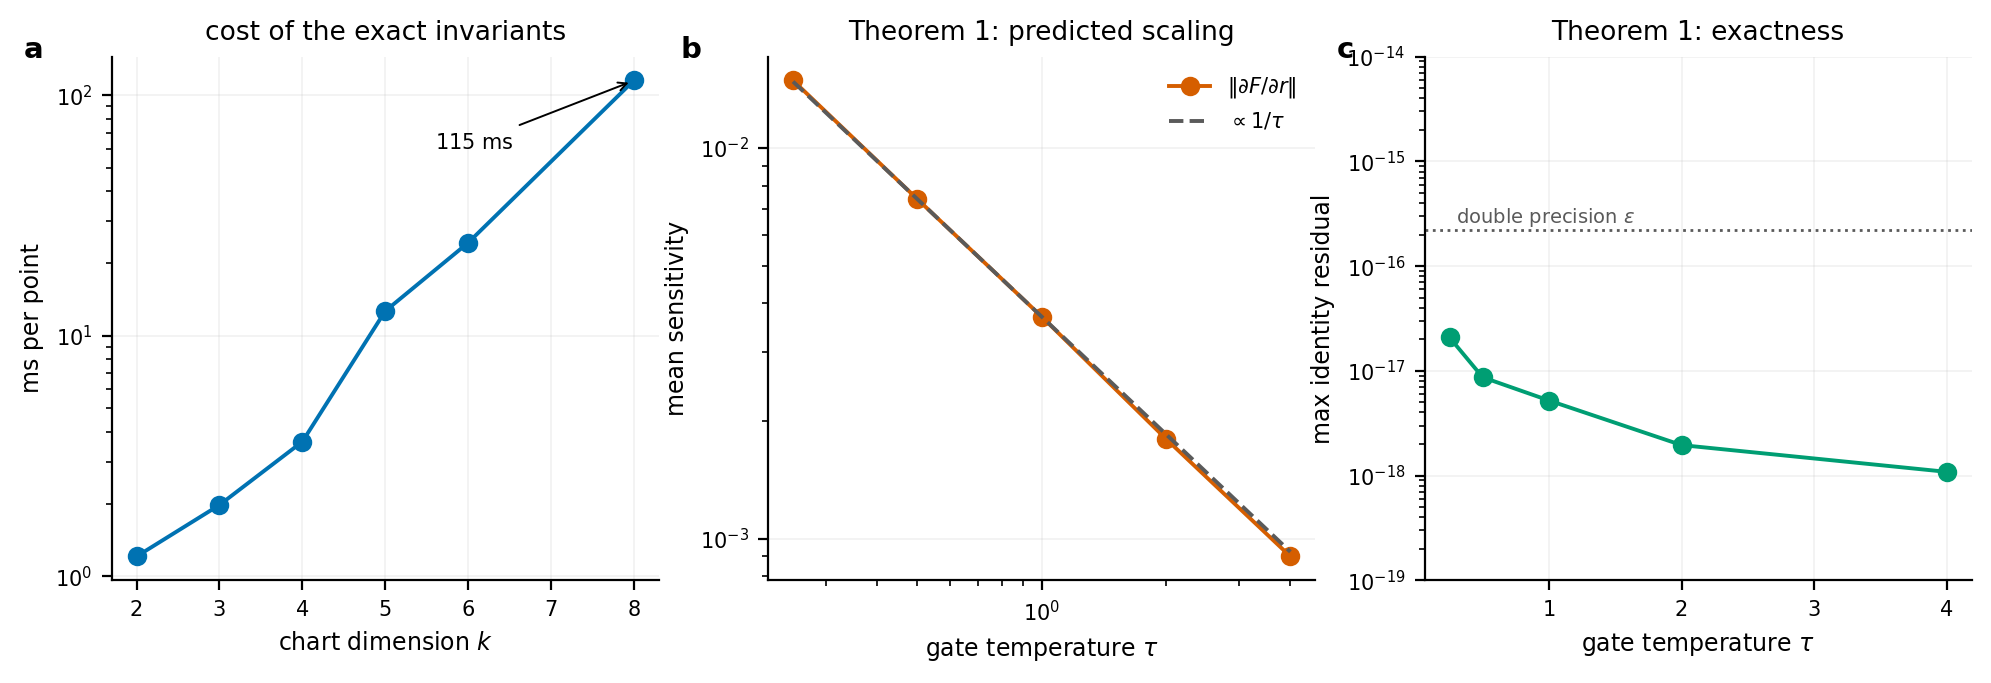
\includegraphics[width=\textwidth]{../figs/f_validation.png}
\caption{\textbf{Validation.} (a) Cost of the exact invariants against chart
dimension; geometry is affordable only on a low-dimensional chart. (b) The
$1/\tau$ scaling of routing sensitivity predicted by Theorem~\ref{thm:sens}.
(c) Residual of the identity \eqref{eq:thm1}, at double-precision epsilon.}
\label{fig:validation}
\end{figure}

\begin{figure}[t]
\centering
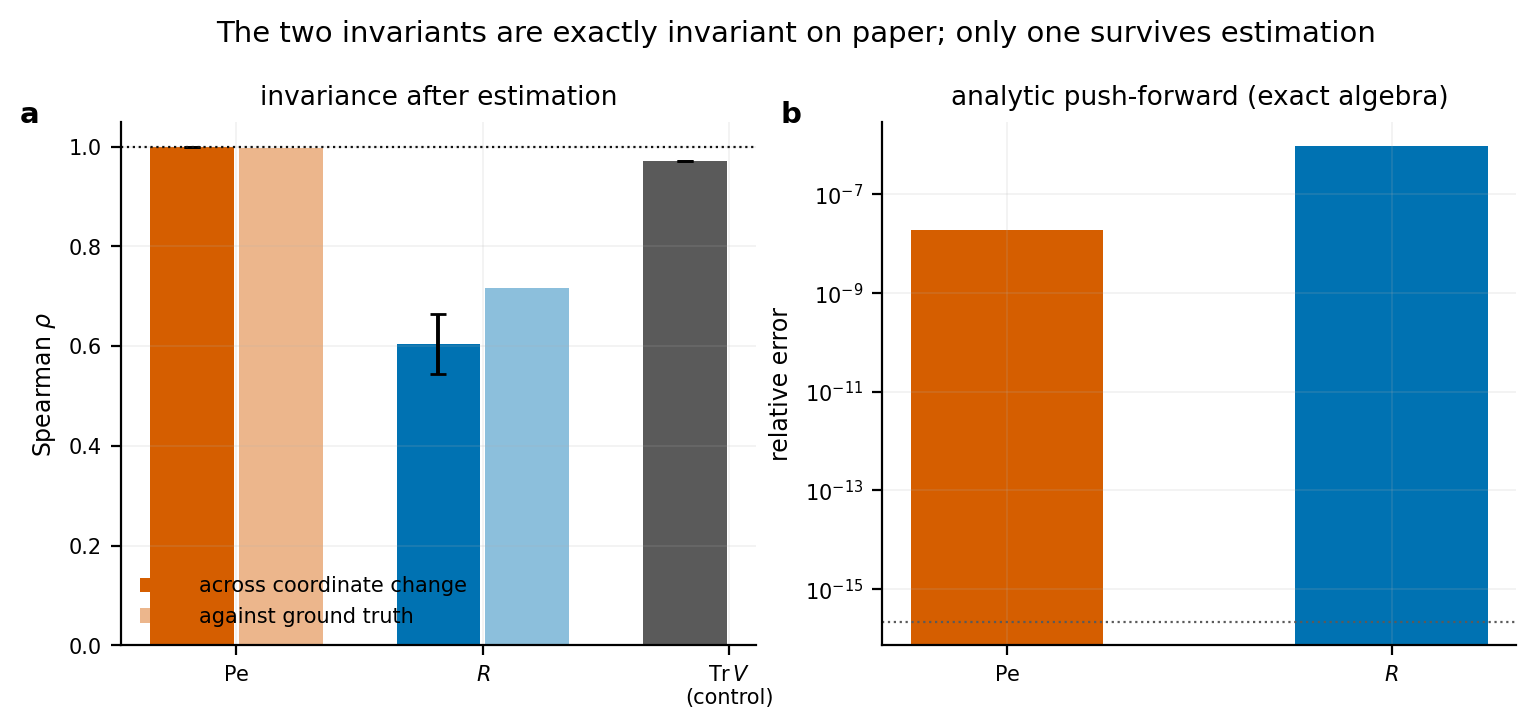
\includegraphics[width=\textwidth]{../figs/f_invariance.png}
\caption{\textbf{Invariance survives estimation for $\Pen$ but not for $R$.}
(a) Spearman agreement of each coordinate across a refit in relabelled
coordinates, and against ground truth. (b) The same quantities computed
analytically, where both are exact.}
\label{fig:invariance}
\end{figure}

\begin{figure}[t]
\centering
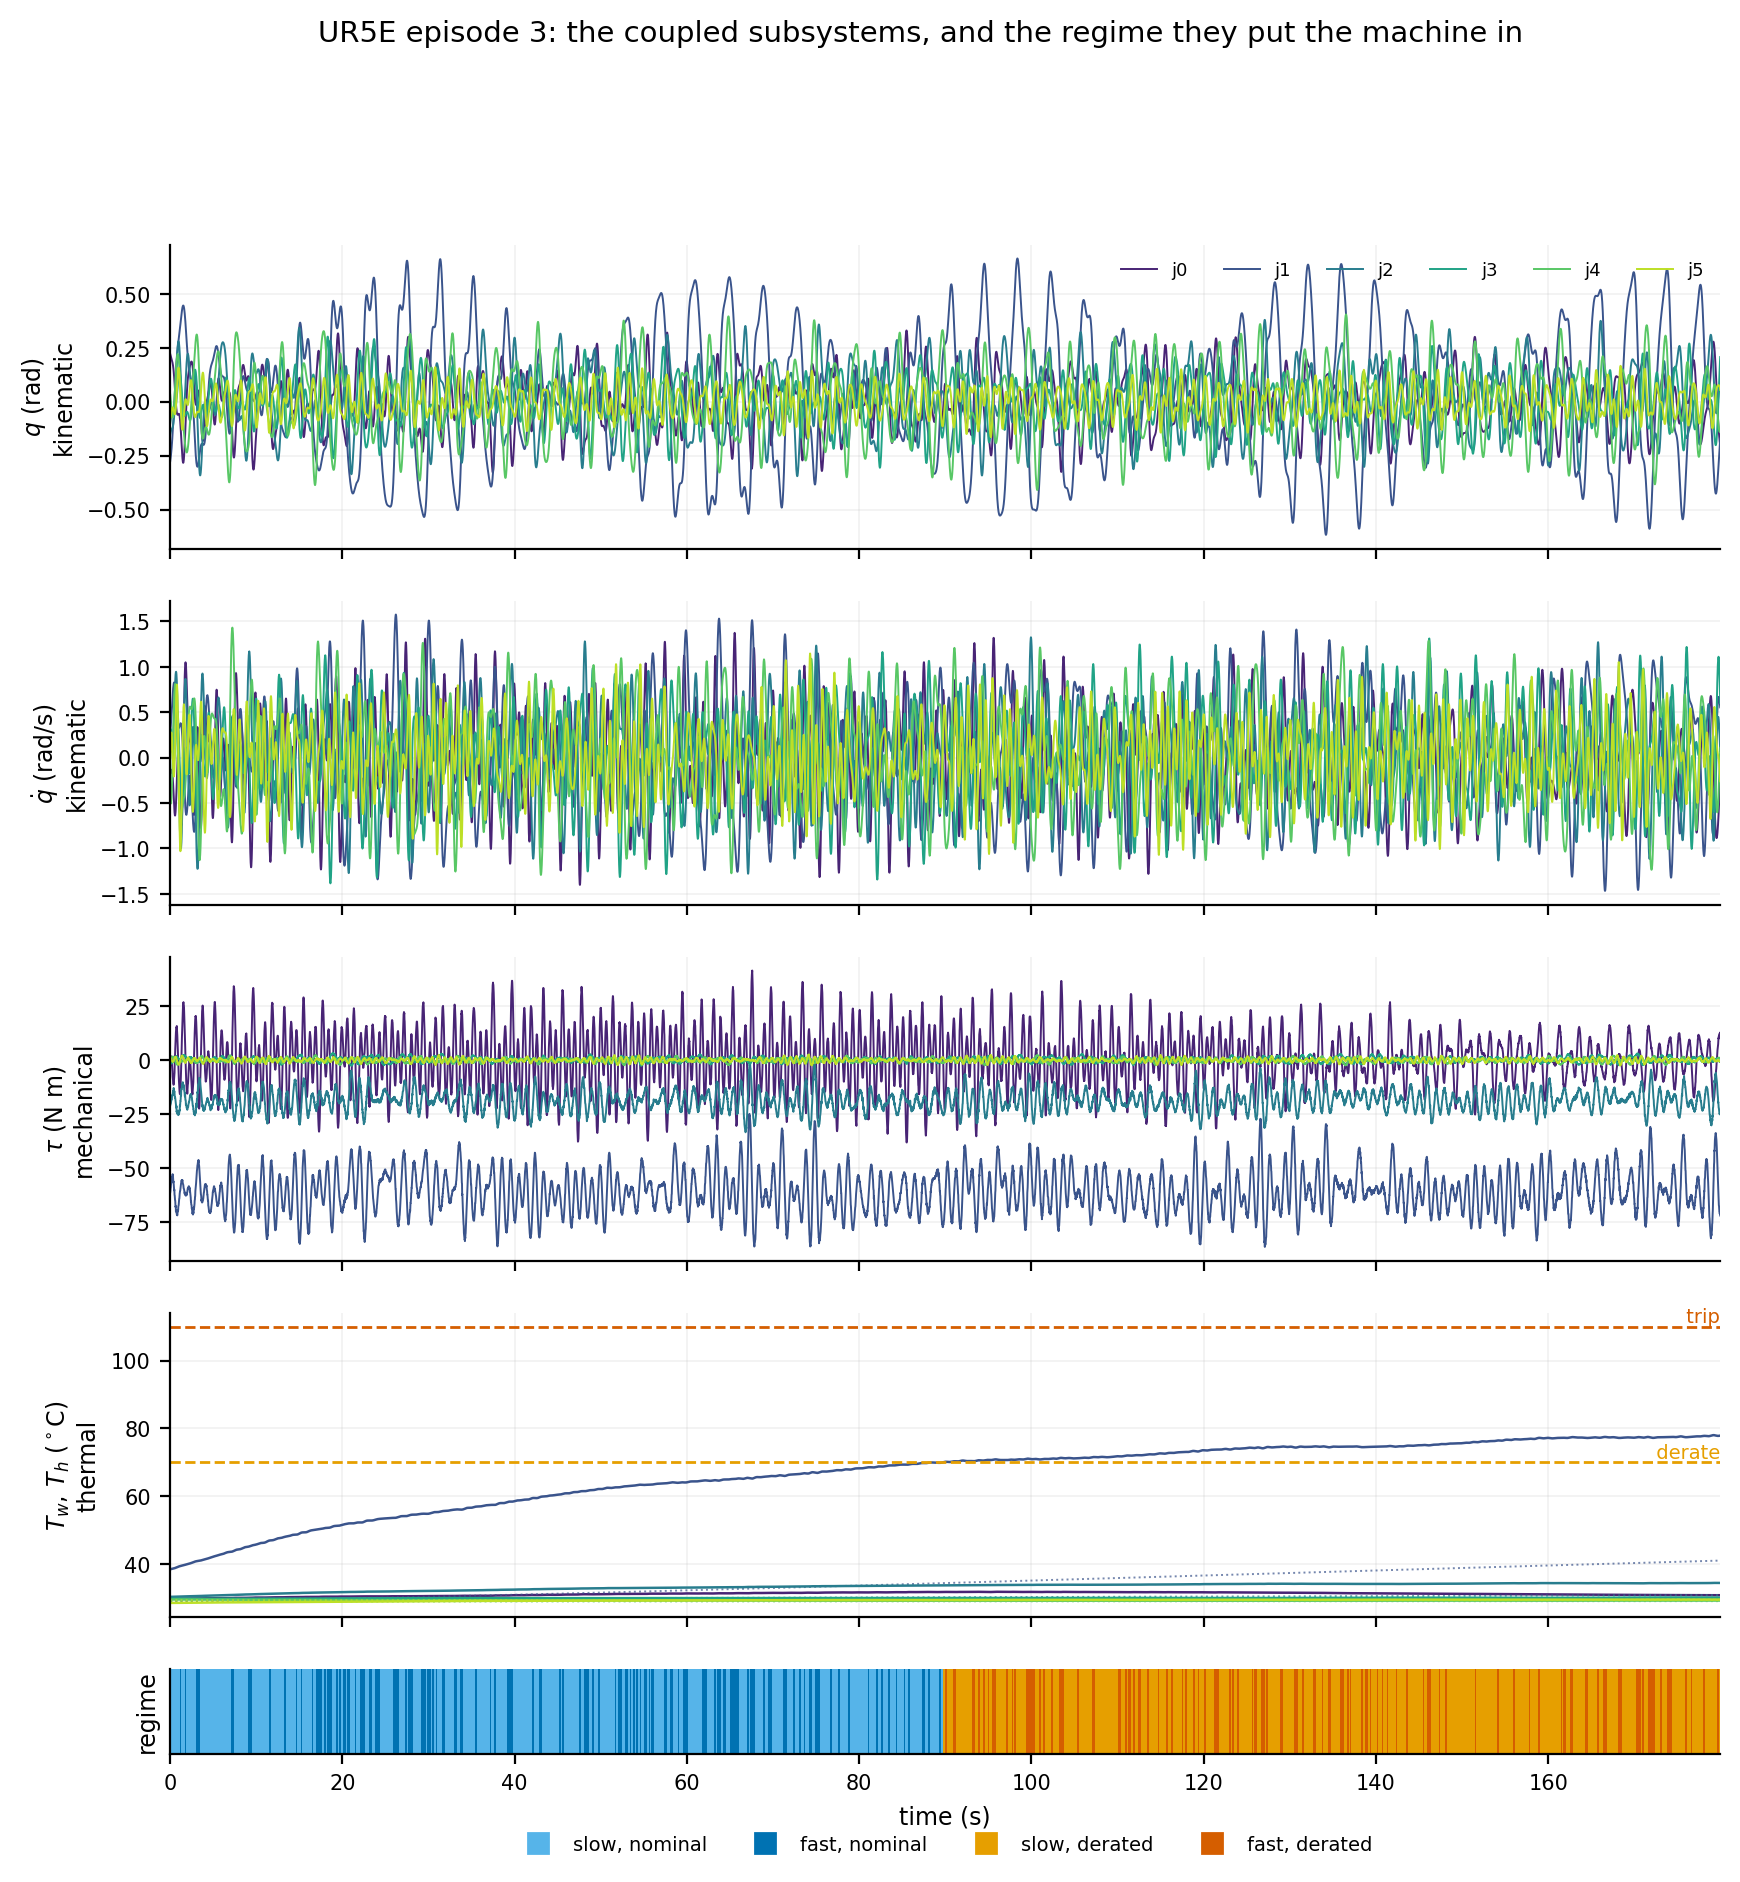
\includegraphics[width=\textwidth]{../figs/f_subsys_ur5e.png}
\caption{\textbf{Coupled subsystems on the UR5e.} Kinematic and mechanical
channels oscillate at $\sim$1\,Hz while joint~1's winding heats over minutes,
crossing the derating knee at $t\approx90$\,s and flipping the ground-truth
regime. The three-decade time-scale separation is the multi-physics coupling.}
\label{fig:subsys}
\end{figure}

\begin{figure}[t]
\centering
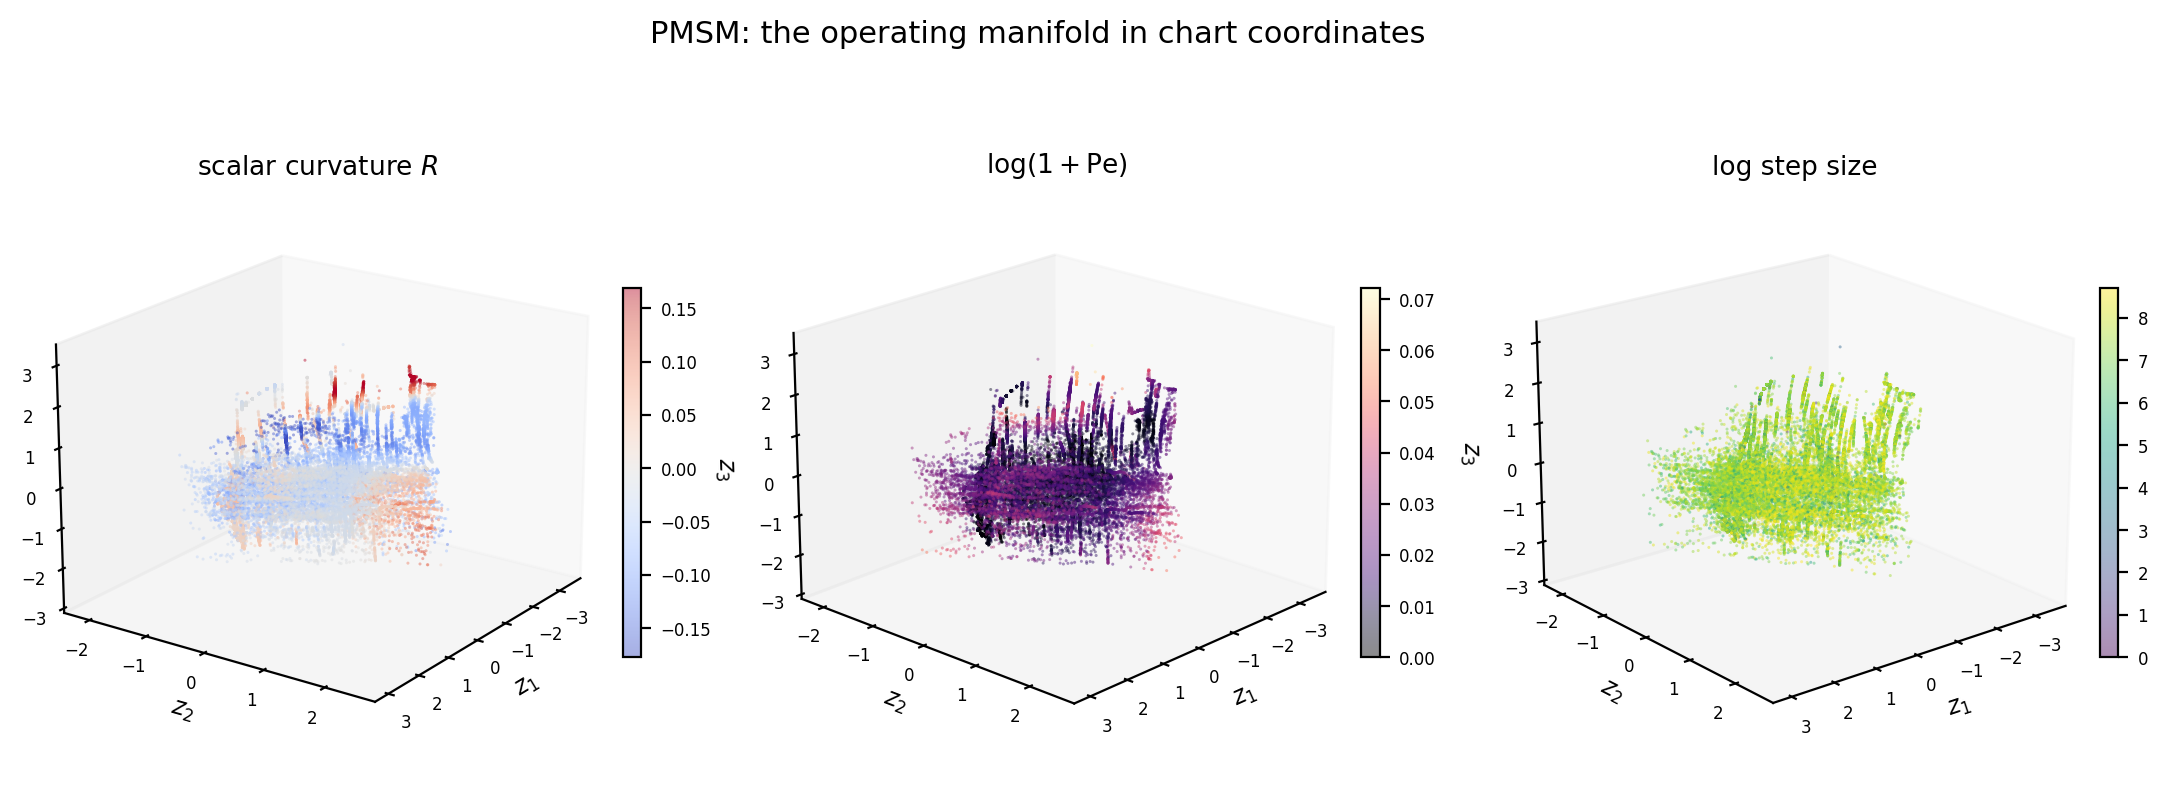
\includegraphics[width=\textwidth]{../figs/f_shape_pmsm.png}
\caption{\textbf{The operating manifold in chart coordinates}, coloured by
scalar curvature, by $\log(1+\Pen)$ and by step size.}
\label{fig:shape}
\end{figure}

\end{document}
